\documentclass[a4paper]{article} %format de la feuille + type de document https://en.wikibooks.org/wiki/LaTeX/Document_Structure#Document_classes
%packages nécessaire pour nos besoins
\usepackage[utf8]{inputenc}
\usepackage[T1]{fontenc}
\usepackage[english,french]{babel}
\usepackage{amsmath}
\usepackage{amssymb,amsfonts,textcomp}
\usepackage{color}
\usepackage{array}
\usepackage{hhline}
\usepackage{hyperref}
\usepackage[pdftex]{graphicx}
\usepackage{sectsty}
\usepackage{tcolorbox}
\usepackage{textcomp}
\usepackage{courier}
\usepackage[font={small,it}]{caption}
\usepackage{float}
\usepackage{graphicx}
\usepackage{caption}
\usepackage{tabularx}
\usepackage{multirow}% http://ctan.org/pkg/multirow
\usepackage{tikz}
\usepackage[top=15mm,bottom=20mm,right=50mm,left=50mm]{geometry} 
\usepackage[export]{adjustbox}


%Définition des couleurs
\definecolor{havelockBlue}{rgb}{0.004, 0.42, 0.73}
\definecolor{Monokaimagenta}{rgb}{0.86,0.08,0.24}

%utilisation de la couleur définie avant
%toutes les sections auront cette couleur
\sectionfont{\color{havelockBlue}}
%\subsectionfont{\color{havelockBlue}}
%début du document
\begin{document}

\renewcommand{\labelitemi}{$\bullet$}
\renewcommand{\labelitemii}{$\cdot$}
\renewcommand{\labelitemiii}{$\diamond$}
\renewcommand{\labelitemiv}{$\ast$}

%début d'un titre
\begin{titlepage}
            %centre les éléments
	\centering
	
	{\scshape\LARGE \color{Monokaimagenta} Laboratoire \\  \par}
	
	%espace vertical de 1 mms
	\vspace{1cm}
	
	{\Large\itshape Sven Rouvinez \& Johanna Melly\par}
	
	%http://www.personal.ceu.hu/tex/spacebox.htm
	\vfill
	Professeur\par
	%met le texte en gras 
	\textbf{Carlos Andrés Pena} \par% ajoute une ligne 
	\vspace{1cm}
	Assistant\par
	\textbf{Gaëtan Matthey}
	
	\vfill

            %affiche la date actuelle
	{\large \today\par}
	
%fin de la page de titre
\end{titlepage}

\section{Objectifs du laboratoire}
La réalisation simplifiée de la partie FETCH d'un processeur RISC\footnote{Reduced Instruction Set Computing} avec l'incrémenation du PC\footnote{Program Counter} et la lecture d'instruction ainsi qu'un mécanisme de saut et un système de gestion d'interruption.

\section{Blocs Logisim}
Nous avons décidé de séparer les blocs afin de permettre une meilleure modularité et abstraction du système FETCH.\\
\paragraph{Résumé}
\begin{itemize}
    \item     MOV\_INST détecte une instruction \textbf{MOV}
    \item     BRANCH\_INST détecte une instruction \textbf{B}
    \item     CALC\_ADR calcule le décalage lors d'une instruction \textbf{B}
    \item     FETCH\_16BITS circuit avec incrémentation du PC et lecture d'instructions
    \item     FETCH\_JUMP\_16BITS circuit avec mécanisme de saut
    \item     FETCH\_INTER\_16BITS (main) circuit avec mécanisme d'interruption
\end{itemize}
\subsection{MOV\_INST}

\begin{figure}[H]
    \centering
    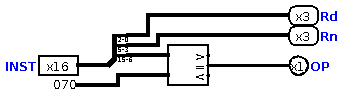
\includegraphics[width=.8\textwidth]{src/MOV_INST.png}
    \caption{Instruction MOV}
    \label{mov}
\end{figure}
\paragraph{Définition des entrées:}
\begin{itemize}
    \item     INST: code complet
    \item     0x70: code recherché
\end{itemize}

\paragraph{Définition des sorties:}
\begin{itemize}
    \item     Rd: registre destination
    \item     Rn: registre source
    \item     OP: s'active si les bits de 15 à 9 sont égal à $0001110$ (0x70)
\end{itemize}

\medskip

Ce bloc permet de détecter si une instruction \textbf{MOV} est trouvée, grâce au comparateur, dans le code de sortie de la ROM, cette instruction va charger le valeur du registre source (Rn) dans le registre destination (Rd).\\
Elle se caractérisque par le code ci-dessous : 
\\
\begin{tabular}{|ccccccc|ccc|ccc|ccc|}
    \hline
    \multicolumn{7}{|c|}{Code ARM}  & \multicolumn{3}{|c|}{Opcode} & \multicolumn{3}{|c|}{Rn} & \multicolumn{3}{|c|}{Rd}\\
    \hline
    15 & 14 & 13 & 12 & 11 & 10 & 9 & 8 & 7 & 6                    & 5 & 4 & 3                & 2 & 1 & 0 \\
    \hline
    0  & 0  & 0  & 1  & 1  & 1  & 0 & 0 & 0 & 0                    & 1 & 0 & 0                & 1 & 0 & 1 \\
    \hline     
    \end{tabular}
\\
\begin{itemize}
    \item     Code ARM : instruction ARM à effectuer
    \item     Opcode : instruction à effectuer par l'ALU
    \item     Rn : registre source
    \item     Rd : registre destination
\end{itemize}


\subsection{BRANCH\_INST}
\begin{figure}[H]
    \centering
    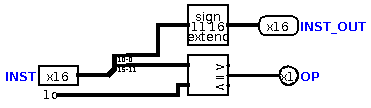
\includegraphics[width=.8\textwidth]{src/BRANCH_INST.png}
    \caption{Instruction BRANCH}
    \label{branch}
\end{figure}

\paragraph{Définition des entrées:}
\begin{itemize}
    \item     INST: code complet
    \item     0x1c: code recherché
\end{itemize}

\paragraph{Définition des sorties:}
\begin{itemize}
    \item     INST\_OUT: contient l'adresse de retour
    \item     Rn: registre source
    \item     OP: s'active si les bits de 15 à 11 sont égal à $00011$ (0x70)
\end{itemize}

\medskip
Grâce à ce bloc, le système sera capable d'effectuer un saut inconditionnel. Pour calculer l'adresse de retour, il faut effectuer une opération: $PC + Adresse*2 + 4$ (voir \ref{bl_calc_adr}).\\

\begin{tabular}{|ccccc|ccccccccccc|}
    \hline
    \multicolumn{5}{|c|}{Code ARM}  & \multicolumn{11}{|c|}{Offset}\\
    \hline
    15 & 14 & 13 & 12 & 11          & 10 & 9 & 8 & 7 & 6 & 5 & 4 & 3 & 2 & 1 & 0 \\
    \hline
    1  & 1  & 1  & 0  & 0           & 1  & 0 & 0 & 0 & 0 & 0 & 0 & 0 & 0 & 0 & 0\\
    \hline     
    \end{tabular}
    \\
\begin{itemize}
    \item     Code ARM : instruction ARM à effectuer
    \item     Offset: adresse relative par rapport au PC
\end{itemize}


\paragraph{Exemple:} dans notre cas, nous avons \textit{B ADR\_SAUT\_1} dans notre fichier d'instructions ce qui équivaut à 0xe7fc. Donc si nous prenons le tableau du haut et que nous faisons la conversion en binaire:
\\
\begin{tabular}{|ccccc|ccccccccccc|}
    \hline
    \multicolumn{5}{|c|}{Code ARM}  & \multicolumn{11}{|c|}{Offset}\\
    \hline
    15 & 14 & 13 & 12 & 11          & 10 & 9 & 8 & 7 & 6 & 5 & 4 & 3 & 2 & 1 & 0 \\
    \hline
    1  & 1  & 1  & 0  & 0           & 1  & 1 & 1 & 1 & 1 & 1 & 1 & 1 & 1 & 0 & 0\\
    \hline     
    \end{tabular}
    
    \medskip
Seul les bits 10 à 0 nous intéresse c'est pourquoi il y a un bit extender de 11 bits $\rightarrow$ 16 bits pour travailler sur la même base.\\
Ensuite nous effectuons le calcul avec un PC à $4$ et un INST\_OUT de 0xfffc: $4 + 1111111111111100 * 2 + 4=0000$ donc l'adresse de retour sera $0000$

\subsection{CALC\_ADR} \label{bl_calc_adr}
\subsection{FETCH\_16BITS}
\subsection{FETCH\_JUMP\_16BITS}
\subsection{FETCH\_INTER\_16BITS}
\section{Fonctionnement global}
\section{Conclusion}
\section{Annexes}

\end{document}